% **************************************************************************************************************
% A Classic Thesis Style
% An Homage to The Elements of Typographic Style
%
% Copyright (C) 2011 Andr\'e Miede http://www.miede.de
%
% If you like the style then I would appreciate a postcard. My address 
% can be found in the file ClassicThesis.pdf. A collection of the
% postcards I received so far is available online at 
% http://postcards.miede.de
%
% License:
% This program is free software; you can redistribute it and/or modify
% it under the terms of the GNU General Public License as published by
% the Free Software Foundation; either version 2 of the License, or
% (at your option) any later version.
%
% This program is distributed in the hope that it will be useful,
% but WITHOUT ANY WARRANTY; without even the implied warranty of
% MERCHANTABILITY or FITNESS FOR A PARTICULAR PURPOSE.  See the
% GNU General Public License for more details.
%
% You should have received a copy of the GNU General Public License
% along with this program; see the file COPYING.  If not, write to
% the Free Software Foundation, Inc., 59 Temple Place - Suite 330,
% Boston, MA 02111-1307, USA.
%
% **************************************************************************************************************
% Note:
%    * You must not use "u etc. in strings/commands that will be spaced out (use \"u or real umlauts instead)
%    * New enumeration (small caps): \begin{aenumerate} \end{aenumerate}
%    * For margin notes: \graffito{}
%    * Do not use bold fonts in this style, it is designed around them
%    * Use tables as in the examples
%    * See classicthesis-ldpkg.sty for useful commands
% **************************************************************************************************************
% To Do:
%    * [high] Check this out: http://www.golatex.de/koma-script-warnung-in-verbindung-mit-listings-package-t2058.html
%    * [medium] mathbb in section-titles/chapter-titles => disappears somehow in headlines!!!
%    * [low] Calculate text block size for Libertine font
%    * [low] Think about processing a4paper, a5paper, 10pt, 11pt, 12pt etc. options for typearea layout
%            (store values in internal variables and handle by \AtEndOfPackage{\areaset...})
% **************************************************************************************************************
\documentclass[ twoside,openright,titlepage,fleqn,numbers=noenddot,headinclude,%1headlines,% letterpaper a4paper
                11pt,a4paper,BCOR5mm,footinclude=true,cleardoublepage=empty,abstractoff % <--- obsolete, remove (todo)
                ]{scrreprt}

% ********************************************************************
% Development Stuff
% ********************************************************************
\listfiles
%\usepackage[l2tabu, orthodox, abort]{nag}
%\usepackage[warning, all]{onlyamsmath}
% ********************************************************************
% Re-usable information
% ********************************************************************
\newcommand{\myTitle}{A Classic Thesis Style\xspace}
\newcommand{\myDegree}{Diplomarbeit\xspace}
\newcommand{\myName}{Max Mustermann\xspace}
\newcommand{\myProf}{Prof. Dr.-Ing. M. Fidler\xspace}
\newcommand{\myOtherProf}{Prof. Dr.-Ing. T. Kaiser\xspace}
\newcommand{\mySupervisor}{Dipl.-Ing. M. Bredel\xspace}
\newcommand{\myFaculty}{Fakult\"{a}t f\"{u}Elektrotechnik und Informationstechnik\xspace}
\newcommand{\myDepartment}{Institut f\"{u}r Kommunikationstechnik\xspace}
\newcommand{\myUni}{\protect{Leibniz Universit\"{a}}t Hannover\xspace}
\newcommand{\myLocation}{Hannover\xspace}
\newcommand{\myTime}{01. Mai 2009\xspace}
\newcommand{\myBirthdate}{01.Januar. 1970\xspace}
\newcommand{\myBirthplace}{Linuxhausen\xspace}
\newcommand{\myVersion}{Version 2.6.1\xspace}
% ********************************************************************
% Packages with options that might require adjustments
% ********************************************************************
\usepackage[latin1]{inputenc} 
\usepackage[ngerman,american]{babel}           
\usepackage[square,numbers]{natbib} 
\usepackage[fleqn]{amsmath} % math environments and more by the AMS 
\usepackage{float} % for H placement specifier
%\usepackage{varioref} % load BEFORE classicthesis-ldpkg
% ********************************************************************
\usepackage{classicthesis-ldpkg} 
% ********************************************************************
% Options for classicthesis.sty:
% tocaligned eulerchapternumbers drafting linedheaders listings
% subfig nochapters beramono eulermath parts minionpro pdfspacing 
% dottedtoc minionprospacing manychapters floatperchapter
\usepackage[eulerchapternumbers,listings,%linedheaders,%pdfspacing,
            subfig,beramono,eulermath,parts,dottedtoc,floatperchapter]{classicthesis}

%*******************************************************
% Some font experiments
%*******************************************************
%\usepackage[osf]{libertine}
%\usepackage{hfoldsty}
%\usepackage[light,condensed,math]{iwona}
%\renewcommand{\sfdefault}{iwona}
%\usepackage{lmodern} % <-- no osf support :-(
%\usepackage[urw-garamond]{mathdesign} <-- no osf support :-(

% ********************************************************************  
% Fine-tuning for the text area
% ********************************************************************  
%\linespread{1.05} % a bit more for Palatino
%\areaset[5mm]{312pt}{761pt} % 686 (factor 2.2) + 33 head + 42 head \the\footskip
%\setlength{\marginparwidth}{7em}%
%\setlength{\marginparsep}{2em}%

% ********************************************************************  
% hack to use citations in float environments 
% will be fixed with caption package version 3.2
% ********************************************************************  
\usepackage{makerobust} 
\makeatletter 
\MakeRobustCommand\caption@xref 
\makeatother 

% ********************************************************************         
% Options for iktthesis.sty:
% abbrev exam big wiwi english
\usepackage[]{iktthesis}
% ********************************************************************
%\usepackage[section,below]{placeins} <--- not everybody wants this
%\usepackage[all]{hypcap} <--- does not work with MiKTeX 2.6
% ********************************************************************
% Language/strings for backrefs (change here, thanks, Lorenzo)
% ********************************************************************
%\renewcommand{\backrefnotcitedstring}{\relax}%(Not cited.)
%\renewcommand{\backrefcitedsinglestring}[1]{(Citato a pagina~#1.)}
%\renewcommand{\backrefcitedmultistring}[1]{(Citato alle pagine~#1.)}
%\renewcommand{\backreftwosep}{ e~}
%\renewcommand{\backreflastsep}{ e~}
% ********************************************************************
% Setup and Finetuning
% ********************************************************************
\newlength{\abcd} % for ab..z string length calculation
\newcommand{\myfloatalign}{\centering} % how all the floats will be aligned
\setlength{\extrarowheight}{3pt} % increase table row height
% ********************************************************************
% Captions look and feel
% ********************************************************************
\captionsetup{format=hang,font=small}
% ********************************************************************
% Listings setup
% ********************************************************************
%\lstset{emph={trueIndex,root},emphstyle=\color{BlueViolet}}%\underbar} % for special keywords
% ********************************************************************
\lstset{language=[LaTeX]Tex,%C++,
    keywordstyle=\color{RoyalBlue},%\bfseries,
    basicstyle=\small\ttfamily,
    %identifierstyle=\color{NavyBlue},
    commentstyle=\color{Green}\ttfamily,
    stringstyle=\rmfamily,
    numbers=none,%left,%
    numberstyle=\scriptsize,%\tiny
    stepnumber=5,
    numbersep=8pt,
    showstringspaces=false,
    breaklines=true,
    frameround=ftff,
    frame=single,
    belowcaptionskip=.75\baselineskip
    %frame=L
} 

% ********************************************************************
% Where to look for graphics
% ********************************************************************
%\graphicspath{{gfx/}{misc/}} % considered harmful according to l2tabu
% ********************************************************************
% Hyperreferences
% ********************************************************************
\hypersetup{%
    colorlinks=true, linktocpage=true, pdfstartpage=3, pdfstartview=FitV,%
    % uncomment the following line if you want to have black links (e.g., for printing)
    %colorlinks=false, linktocpage=false, pdfborder={0 0 0}, pdfstartpage=3, pdfstartview=FitV,% 
    breaklinks=true, pdfpagemode=UseNone, pageanchor=true, pdfpagemode=UseOutlines,%
    plainpages=false, bookmarksnumbered, bookmarksopen=true, bookmarksopenlevel=1,%
    hypertexnames=true, pdfhighlight=/O,%hyperfootnotes=true,%nesting=true,%frenchlinks,%
    urlcolor=webbrown, linkcolor=RoyalBlue, citecolor=webgreen, %pagecolor=RoyalBlue,%
    % uncomment the following line if you want to have black links (e.g., for printing)
    %urlcolor=Black, linkcolor=Black, citecolor=Black, %pagecolor=Black,%
    pdftitle={\myTitle},%
    pdfauthor={\textcopyright\ \myName, \myUni, \myFaculty},%
    pdfsubject={},%
    pdfkeywords={},%
    pdfcreator={pdfLaTeX},%
    pdfproducer={LaTeX with hyperref and classicthesis}%
}
% ********************************************************************
% Hyphenation
% ********************************************************************
%\hyphenation{put special hyphenation here}
% ********************************************************************
% GO!GO!GO! MOVE IT!
% ********************************************************************
\begin{document}
\frenchspacing
\raggedbottom
\selectlanguage{ngerman} % american ngerman
%\renewcommand*{\bibname}{new name}
%\setbibpreamble{}
\pagenumbering{roman}
\pagestyle{plain}
% ********************************************************************
% Frontmatter
% ********************************************************************
%*******************************************************
% Titlepage
%*******************************************************
%%%
%%% title page (german)
%%%
\pdfbookmark[0]{Titelblatt}{title}
\begin{titlepage}
  \changetext{}{19mm}{}{19mm}{}
  \vspace{1cm}
  \begin{center}
    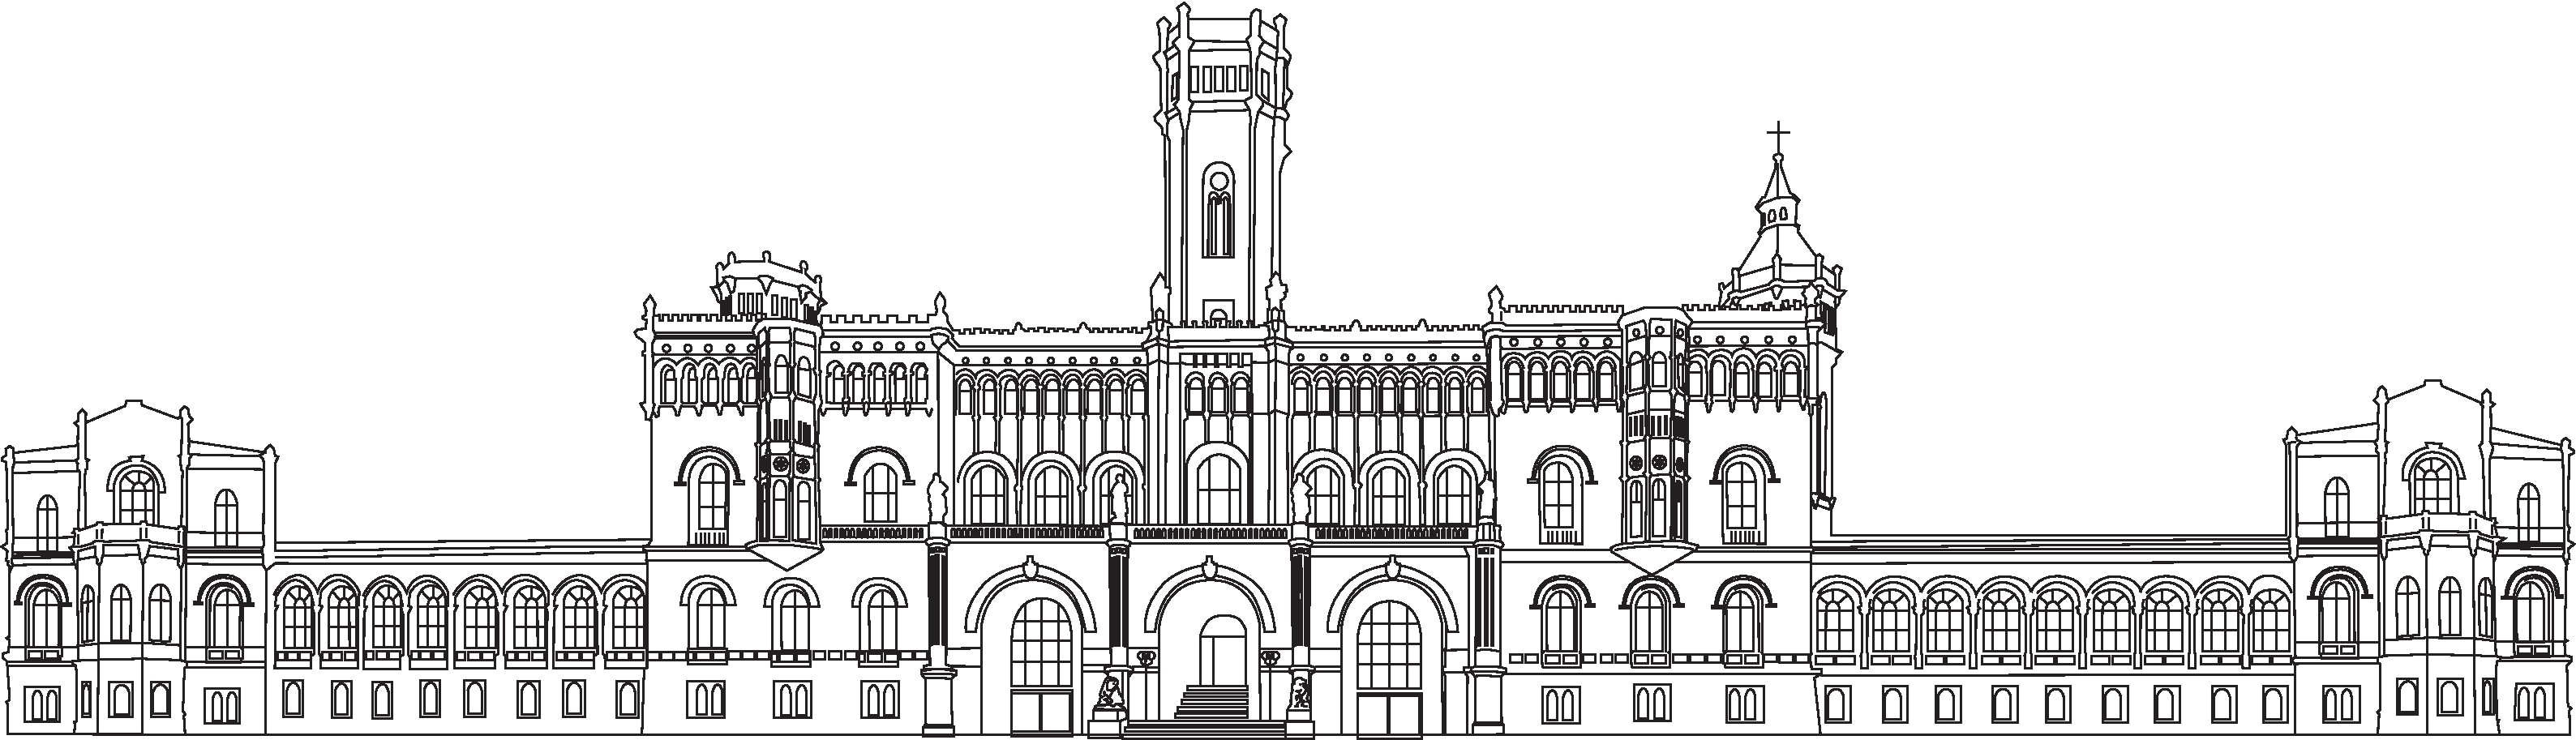
\includegraphics[width=13.8cm]{gfx/welfenschloss} \\ 
  \end{center}
  \medskip
  \begin{center}
    \textbf{\huge\spacedallcaps{L}\LARGE\spacedallcaps{eibniz}}
    \textbf{\huge\spacedallcaps{U}\LARGE\spacedallcaps{niversit\"{a}t}}
    \textbf{\huge\spacedallcaps{H}\LARGE\spacedallcaps{annover}} \\
  \end{center}

  \begin{center}
    \normalsize
    \spacedallcaps{Fakult\"{a}t}
    \spacedallcaps{f\"{u}r}
    \spacedallcaps{Elektrotechnik}
    \spacedallcaps{und}
    \spacedallcaps{Informatik} \\
    \smallskip
    \spacedallcaps{Institut}
    \spacedallcaps{f\"{u}r}
    \spacedallcaps{Kommunikationstechnik}
  \end{center}
  \vfill
  \vfill

  % Start condWIWI
  \condWIWI{
  %*******************************************************
  % Titlepage for Wirtschaftingenieur
  %*******************************************************
  \begin{center}
    \Large \myTitle
  \end{center}
  \vfill
  \vfill

  \begin{center}
    \LARGE \textbf{\myDegree}
  \end{center}
  \vfill

  \begin{center}
    \large zur Erlangung des Grades eines Diplom-Wirtschaftsingenieurs der \\
    \large Fakult\"{a}t f\"{u}r Elektrotechnik und Informatik, Fakult\"{a}t f\"{u}r Maschinenbau und \\
    \large Wirtschaftswissenschaftlichen Fakult\"{a}t der Leibniz Universit\"{a}t Hannover
  \end{center}
  \vfill

  \begin{center}
    \large vorgelegt von \\
  \end{center}
  \medskip

  \begin{center}
    \large \spacedallcaps{\myName}
  \end{center}
  \medskip

  \begin{center}
    \large geb. am \myBirthdate in \myBirthplace \\
  \end{center}

  \vfill
  \vfill

  Pr\"{u}fer: \myProf
  \bigskip

  Hannover, den \myTime
  } 
  {
  %*******************************************************
  % Titlepage for everyone else 
  %*******************************************************
  \begin{center}
    \LARGE \myTitle
  \end{center} 
  \vfill
  \vfill

  \begin{center}
    \LARGE \textbf{\myDegree}
  \end{center}
  \vfill

  \begin{center}
    \large eingereicht von \\
  \end{center}

  \begin{center}
    \large \spacedallcaps{\myName}
  \end{center}

  \begin{center}
    \large am \myTime \\
  \end{center} 
  \vfill

  \begin{center}
    \begin{tabular}{lll}
      Erstpr\"{u}fer  & : & \myProf \\
      Zweitpr\"{u}fer & : & \myOtherProf \\
      Betreuer        & : & \mySupervisor
    \end{tabular}
  \end{center} 

  }  % end condWIWI

%  \vfill

%  \begin{center}
%    \large \selectedthesisnumber \\
%  \end{center}

  \changetext{}{-19mm}{}{-19mm}{}

\end{titlepage}

\thispagestyle{empty}

\hfill

\vfill

\noindent\myName: \textit{\myTitle,} \myDegree, \textcopyright\ \myTime

%\bigskip
%
%\noindent\spacedlowsmallcaps{Supervisors}: \\
%\myProf \\
%\myOtherProf \\ 
%\mySupervisor
%
%\medskip
%
%\noindent\spacedlowsmallcaps{Location}: \\
%\myLocation
%
%\medskip
%
%\noindent\spacedlowsmallcaps{Time Frame}: \\
%\myTime

\cleardoublepage%*******************************************************
% Declaration
%*******************************************************
\refstepcounter{dummy}
\pdfbookmark[1]{Ehrenw\"{o}rtliche Erkl\"{a}rung}{ehrenw\"{o}rtliche erkl\"{a}rung}
\chapter*{Ehrenw\"{o}rtliche Erkl\"{a}rung}
\thispagestyle{empty}

% Start condWIWI
\condWIWI{
%*******************************************************
% Declaration for Wirtschaftingenieur
%*******************************************************
Hiermit versichere ich, dass ich die vorliegende Arbeit selbstst\"{a}ndig verfasst und keine anderen als die angegebenen Quellen und Hilfsmittel benutzt habe, dass alle Stellen der Arbeit, die w\"{o}rtlich oder sinngem\"{a}\ss aus anderen Quellen \"{u}bernommen wurden, als solche kenntlich gemacht sind und dass die Arbeit in gleicher oder \"{a}hnlicher Form noch keiner Pr\"{u}fungsbeh\"{o}rde vorgelegt wurde.
}
{
%*******************************************************
% Delcaration for everyone else 
%*******************************************************
Hiermit versichere ich, die vorliegende \myDegree ohne Hilfe Dritter und nur mit den angegebenen Quellen und Hilfsmitteln angefertigt zu haben. Alle Stellen, die w\"{o}rtlich oder inhaltlich aus den Quellen entnommen wurden, sind als solche kenntlich gemacht worden. Diese Arbeit hat in gleicher oder \"{a}hnlicher Form noch keiner Pr\"{u}fungsbeh\"{o}rde vorgelegen.
} % end condWIWI

\bigskip
 
\noindent\textit{\myLocation, den \myTime}

\smallskip

\begin{flushright}
    \begin{tabular}{m{5cm}}
        \\ \hline
        \centering\myName \\
    \end{tabular}
\end{flushright}

\cleardoublepage%*******************************************************
% Abstract
%*******************************************************
%\renewcommand{\abstractname}{Abstract}
\pdfbookmark[1]{Abstract}{Abstract}
\begingroup
\let\clearpage\relax
\let\cleardoublepage\relax
\let\cleardoublepage\relax

\chapter*{Abstract}
In this thesis I will give an introduction to recommender systems, provide an overview over other recommender system libraries and datasets available to try out the algorithms. After that I will describe different recommender algorithms and evaluation metrics I implemented in my work followed by an explanation on how to use them. Additionally I will provide the result of the tests.


\vfill

\pdfbookmark[1]{Zusammenfassung}{Zusammenfassung}
\chapter*{Zusammenfassung}
Kurze Zusammenfassung des Inhaltes in deutscher Sprache\dots


\endgroup			

\vfill

\cleardoublepage
\pagestyle{scrheadings}
\cleardoublepage%*******************************************************
% Table of Contents
%*******************************************************
%\phantomsection
\refstepcounter{dummy}
\pdfbookmark[1]{\contentsname}{tableofcontents}
\setcounter{tocdepth}{2} % <-- 2 includes up to subsections in the ToC
\setcounter{secnumdepth}{3} % <-- 3 numbers up to subsubsections
\manualmark
\markboth{\spacedlowsmallcaps{\contentsname}}{\spacedlowsmallcaps{\contentsname}}
\tableofcontents 

\cleardoublepage

\cleardoublepage%*******************************************************
% List of Figures
%*******************************************************    
\automark[section]{chapter}
\renewcommand{\chaptermark}[1]{\markboth{\spacedlowsmallcaps{#1}}{\spacedlowsmallcaps{#1}}}
\renewcommand{\sectionmark}[1]{\markright{\thesection\enspace\spacedlowsmallcaps{#1}}}
%\phantomsection 
\refstepcounter{dummy}
%\addcontentsline{toc}{chapter}{\listfigurename}
\pdfbookmark[1]{\listfigurename}{lof}
\listoffigures

\vspace*{8ex}

\cleardoublepage

\cleardoublepage%*******************************************************
% List of Tables
%*******************************************************
\automark[section]{chapter}
\renewcommand{\chaptermark}[1]{\markboth{\spacedlowsmallcaps{#1}}{\spacedlowsmallcaps{#1}}}
\renewcommand{\sectionmark}[1]{\markright{\thesection\enspace\spacedlowsmallcaps{#1}}}
%\phantomsection 
\refstepcounter{dummy}
%\addcontentsline{toc}{chapter}{\listtablename}
\pdfbookmark[1]{\listtablename}{lot}
\listoftables

\vspace*{8ex}

\cleardoublepage
\cleardoublepage%*******************************************************
% List of Listings
%*******************************************************      
\automark[section]{chapter}
\renewcommand{\chaptermark}[1]{\markboth{\spacedlowsmallcaps{#1}}{\spacedlowsmallcaps{#1}}}
\renewcommand{\sectionmark}[1]{\markright{\thesection\enspace\spacedlowsmallcaps{#1}}}
%\phantomsection 
\refstepcounter{dummy}
%\addcontentsline{toc}{chapter}{\lstlistlistingname}
\pdfbookmark[1]{\lstlistlistingname}{lol}
\lstlistoflistings

\vspace*{8ex}

\cleardoublepage

\cleardoublepage%*******************************************************
% Acronyms
%*******************************************************
\automark[section]{chapter}
\renewcommand{\chaptermark}[1]{\markboth{\spacedlowsmallcaps{#1}}{\spacedlowsmallcaps{#1}}}
\renewcommand{\sectionmark}[1]{\markright{\thesection\enspace\spacedlowsmallcaps{#1}}}
%\phantomsection 
\refstepcounter{dummy}
\pdfbookmark[1]{Abk\"{u}rzungsverzeichnis}{abk\"{u}rzungsverzeichnis}
\markboth{\spacedlowsmallcaps{Abk\"{u}rzungsverzeichnis}}{\spacedlowsmallcaps{Abk\"{u}rzungsverzeichnis}}
\chapter*{Abk\"{u}rzungsverzeichnis}

% Insert your acronyms here
\begin{acronym}[UML]
  \acro{DRY}{Don't Repeat Yourself}
  \acro{API}{Application Programming Interface}
  \acro{UML}{Unified Modeling Language}
\end{acronym}

\cleardoublepage

% ********************************************************************
% Mainmatter
% ********************************************************************
\pagenumbering{arabic}
% use \cleardoublepage here to avoid problems with pdfbookmark
% insert your chapters here
\cleardoublepage\part{Beispiel einer Arbeit}
\chapter{Introduction}


\section{Motivation}

The library together with this document shall provide a ``cookbook''
for recommender systems. With the simple syntax and the interactivity
of Python it is aimed at beginners to simply experiment with different
algorithms. Especially the interactivity is missing in the already
existing libraries because none of them is written in Python.


\section{Task (what a Recommender System does)}

A Recommender System works in a scenario with users, items and interactions
users can have with items. Such a scenario could be an online shop,
where the interactions are purchases of items by users or a video
platform, where the users interact with items (videos) by watching
them. Based on the past interactions of the users a Recommender System
searches for items a user haven't interacted with yet but the probability
that he will interact is maximized.

The interactions can be implicit like purchases or clicks, then the
scenario is also called item prediction. When the feedback is provided
explicit like ratings the scenario is called rating prediction. In
this work the focus lies on implicit feedback or item prediction.
However ratings can be interpreted as the strength of implicit feedback.
For example how often a user purchased an item. Some algorithms implemented
in this library can use this information but none will explicitly
predict ratings like it's usual in rating prediction scenarios.


\section{Contributions}

The main contribution of my work is the interactive library I wrote
\cite{recsyslab}. Also in this document I provide explanations about
the algorithms implemented in the library and an extensive user manual
of the library.



\chapter{Background}
In this chapter we will provide a short overview over the techniques
used to evaluate recommender algorithms.


\section{Evaluation Methods}

To evaluate a recommender algorithm we have to split up the database
into one for training and one for evaluation. There are different
methods to split the database but in the library only one is implemented
which is the Leave-one-out protocol~\cite{leaveoneout}.
You can use the Leave-one-out protocol with many different metrics
which are also explained here.


\subsection{Leave-one-out Protocol}
\label{leaveoneout}

The Leave-one-out protocol means, that we take one interaction of
each user out of the database for training and use it for validation.
The item the recommender has to predict is also called hidden item. 
Now we can test for each user if the algorithm is capable to predict
this missing interaction. Most of the test metrics described below are counting
how many of the hidden items the algorithm recommends while being
restricted to only recommend a certain number of items. But all
of them take recommendations for each user. This wouldn't be possible
if we would for example just take out 1\% of the interactions it's
likely that there are some users without a hidden item. Then the metrics
wouldn't work anymore.



\subsection{Evaluation metrics}
\label{evaluationmetrics}

These are a selection of different metrics to rate the recommendations.
By default the evaluations are executed with only one hidden item
but generally the metrics should also work with more than just one.

For the notation: U is the set of users, H is the set of hidden items
and \(H_u\) is the set of hidden items for user u. T is the set used for 
training. \(\text{TopN}_u\)
is the set of top N recommendations for user u so the number of items
the recommender is allowed to recommend is N. For the metrics where
the order in which the items are recommended count \(\text{TopN}_u\)
is a list sorted by score in decreasing order.
To get an implicit score of each item the recommender recommends all
items.


\subsubsection{Hitrate/Recall@N}

This metrics lets the recommender recommend N items. If the hidden
item is under the N recommended items, the recommender got a 
hit~\cite{Karypis:2001:EIT:502585.502627, Sarwar00applicationof}.
So the Recall@N is the fraction of users who get recommended a
relevant item when the recommender can recommend N items.
So the hitrate is 

\begin{equation} 
\text{Recall@N}=\frac{\sum_{u \in U} H_u \cap \text{topN}_u}{|H|}
\end{equation}


This metric is very intuitive you can for example imagine that you
show the user 10 items then Recall@10 would be the chance of showing
the user an item he will interact with. But this metric doesn't take
the number of recommended items into account.


\subsubsection{Precision}

The precision~\cite{Sarwar00applicationof} is 

\begin{equation} 
\text{Precision}=\frac{\sum_{u \in U} H_u \cap \text{topN}_u}{N \times |U|}
\end{equation}


As you can clearly see this metric is taken the number of recommended
items into account. Which will probably lead to worse results as the
number of recommended items increases.


\subsubsection{F1}

The F1 metric~\cite{Sarwar00applicationof} tries to balance hitrate and precision
by taking both into account.

\begin{equation}
\text{F1}=\frac{2 \times \text{Recall@N} \times \text{Precision}}{\text{Recall@N} + \text{Precision}}
\end{equation}


\subsubsection{Mean Reciprocal Hitrate}

The mean reciprocal hitrate or more general mean reciprocal
rank~\cite{DBLP:conf/icdm/NingK11} counts the hits but punishes them the more the lower they
appear in the list of recommendations. So if the hidden item appears
first in the list of recommendations the hit counts as one, but when
it is in the second position the hit already counts only as one half
and so on.

\begin{equation}
\text{MRHR}=\frac{1}{|U|} \sum_{u \in U} \frac{1}{\text{pos}(\text{topN}_{u},H_{u})}
\end{equation}

Where N is the number of items in the dataset and \(\text{pos}(\text{topN}_{u},H_{u})\)
is the position of the hidden item in the recommendation.


\subsubsection{Area under the ROC (AUC)}

AUC~\cite{Rendle:2009:BBP:1795114.1795167} counts the number of items the recommender rates
higher than the hidden item, normalize it by the number of items the
recommender can rate higher. Sum this up for every user and again
normalize by the number of users.

To get an implicit score of each item the recommender recommends all
items in a list sorted by score in decreasing order. This is in fact the same
as for the other metrics only that the recommender can recommend as
many items as possible.

\begin{equation}
\text{AUC}=\frac{1}{|U|}\sum_{u \in U} \frac{1}{|E(u)|} \sum_{(i,j) \in E(u)} \delta(x_{ui}>x_{uj})
\end{equation}

Where \(x_{ui}\) is the predicted score of the interaction between User u and item i.
\(\delta\) is defined as follows
\begin{equation}
\delta(x)=\begin{cases}1, & \text{if x is true} \\
                       0, & \text{otherwise}
\end{cases}
\end{equation}

And \(E(u)\) is 
\begin{equation}
E(u) =\{(i,j)|(u,i) \in H \land (u,j) \not\in (H \cup T)\}
\end{equation}


\section{Datasets for testing}

In the WWW there are several anonymized datasets available to try
out recommender systems and to evaluate their performance. 
Following we will introduce three of them.


\subsection{MovieLens}
\label{movielens}

MovieLens~\cite{movielensdatasets} is a database provided by GroupLens, a research
lab at the University of Minnesota. One of their research areas is
recommender systems and they built an application where users rate
movies and then get recommendations for movies the could like. The
MovieLens dataset is the ratings gathered by this application. For
this work we will interpret the rating as intensity of interaction
between users and items for example the number of times the user saw
this movie.

The dataset is available in three different sizes:
\begin{itemize}
\item 100,000 interactions
\item 1 million interactions
\item 10 million interactions
\end{itemize}
For the experiments the smallest dataset is totally sufficient, with
the larger datasets the computation time gets too long for just trying
something out.


\subsection{Million Song Dataset}
The million song dataset~\cite{Bertin-Mahieux2011} is a large database of features and media data
of a million songs. For a challenge they also provided the listening history of over 1 million
user. To present I will use a subset of this dataset to keep the computing time required
reasonable low so it's easier for others to retrace the results.


\subsection{476 Million Twitter Tweets Dataset}
The Stanford Network Analysis Project provided a twitter dataset with about 467 million tweets from 17.000 users~\cite{snap}.
Unfortunately the dataset is no more available. [further explanation or deletion]
To convert the tweets two user item interactions I will interpret the hashtags[explanation necessary?] as items.
So tweets of a user with a hashtag is a interaction between the user and the hashtag.


\chapter{Related Work}
\label{relatedwork}

There is a wide range of projects providing implementations for recommender
system. Some of them are described in this chapter to give a quick
overview and comparison.


\section{MyMediaLite}

MyMediaLite~\cite{Gantner2011MyMediaLite} is an open source project developed at the
University of Hildesheim and provides several algorithms for rating
prediction and item prediction. It is written in C\# and can be used with
a command line interface. It also provides a graphical interface to
demonstrate recommender algorithms.


\section{PREA (Personalized Recommendation Algorithms Toolkit)}

PREA~\cite{2012arXiv1205.3193L} is an open source project written in Java. It provides
a wide range of recommender algorithms and evaluation metrics to test
them. It is maintained by the Georgia Institute of Technology.


\section{Apache Mahout}

Mahout~\cite{mahout} is an open source library in Java. It is implemented
on top of Apache Hadoop, so it uses the map/reduce paradigm. This
means it can run on different, independent computers.


\section{Duine Framework}

The Duine Framework~\cite{duine} is an open source project written
in Java by the Telematica Instituut/Novay. The recommender of the
Duine Framework combines multiple prediction techniques to exploit
the strengths of the different techniques and to avoid their weaknesses.


\section{Cofi}

Cofi~\cite{cofi} provides an algorithm for the rating prediction
task called Maximum Margin Matrix Factorization. It is open source
and written in C++.


\section{LensKit}

Lenskit~\cite{Ekstrand:2011:RRR:2043932.2043958} is a toolkit which provides several recommender
algorithms and an infrastructure to evaluate them. It is an open source
project by the University of Minnesota.


\section{Comparison}
The table below compares the algorithms implemented by the different
frameworks.

\begin{table}[h]
\scalebox{0.53}{
\begin{tabular}{c|l|cccccc} \toprule
    Category & Feature & PREA & Mahout & Duine & Cofi & MyMedia & \textbf{recsyslab}\\ \midrule
    \multirow{2}{*}{Baselines} & Constant & O & & & O & O & O\\
                               & User/Item Average & O & O & O &O&O& \\
                               & Random &O&&&&O&O\\\midrule
    \multirow{3}{*}{Memory-based CF}& User-based CF~\cite{su2009survey}&O&O&O&O&O&O\\
                                    & Item-based CF~\cite{linden2003amazon}&O&O&O&O&O&O\\
                                    & Default Vote, Inf-User-Frex~\cite{breese1998empirical}&O&O&&&&\\
                                    & Slope-One~\cite{lemire2005slope}&O&O&&&O&O\\ \midrule
    \multirow{6}{*}{Matrix Factorization}&SVD~\cite{paterek2007improving}&O&O&&O&O&O\\
                                         &NMF~\cite{seung2001algorithms}&O&&&&&\\
                                         &PMF~\cite{salakhutdinov2008probabilistic}&O&&&&&\\
                                         &Bayesian PMF~\cite{salakhutdinov2008bayesian}&O&&&&&O\\
                                         &Non-linear PMF~\cite{lawrence2009non}&O&&&&&\\
                                         &RankMFX~\cite{diaz2012happening}&&&&&&O\\ \midrule
    \multirow{2}{*}{Other methods}       &Fast NPCA~\cite{yu2009fast}&O&&&&&\\
                                         &Rank-based CF~\cite{sun2012estimating}&O&&&&&\\ \midrule
    \multirow{5}{*}{Evaluation Metric}   &(N)MAE&O&O&O&O&O&\\
                                         &RMSE&O&O&&O&O&\\
                                         &HLU/NDCG&O&&&&O&\\
                                         &Kendall's Tau, Spearman&O&&&&&\\
                                         &Precision/Recall/F1&&O&&&O&O\\
                                         &ARHR/MRHR&&&&&&O\\ \midrule
    \multirow{6}{*}{Miscelaneous}        &Sparse Vector/Matrix&O&O&O&O&O&O\\
                                         %&Wrapper for other languages&O&&&O&O&\\
                                         &Item Recommender for Positive-only Data&&&&&O&O\\
                                         &Release Year&2011&2005&2009&2004&2009&2013\\
                                         &Language&Java&Java&Java&C++&C\#&Python\\
                                         &License&GPL&LGPL&LGPL&GPL&GPL&GPLv3\\ \bottomrule
\end{tabular}}
\label{comparisontable}
\caption{Comparison of different recommender frameworks}
\end{table}

% ********************************************************************
% Backmatter
% ********************************************************************
\appendix
% insert your appendix here
\cleardoublepage\part{Appendix - Some Kind of Manual}
%************************************************
\chapter{Introduction to the ClassicThesis style}\label{ch:introduction}
%************************************************
This bundle for \LaTeX\ has two goals:
\begin{enumerate}
    \item Provide students with an easy-to-use template for their
    Master's
    or PhD thesis. (Though it might also be used by other types of
    authors
    for reports, books, etc.)
    \item Provide a classic, high quality typographic style which is
    inspired by \cauthor{bringhurst:2002}'s ``\emph{The Elements of
    Typographic Style}'' \citep{bringhurst:2002}.
    \graffito{\myTitle \myVersion}
\end{enumerate}
The bundle is configured to run with a \emph{full} 
MiK\TeX\ or \TeX Live\footnote{See the file \texttt{LISTOFFILES} for
needed packages. Furthermore, \texttt{classicthesis} 
works with most other distributions and, thus, with most operating 
systems \LaTeX\ is available for.} 
installation right away and, therefore, it uses only freely available 
fonts. (Minion fans can easily adjust the style to their needs.)

People interested only in the nice style and not the whole bundle can
now use the style stand-alone via the file \texttt{classicthesis.sty}.
This works now also with ``plain'' \LaTeX.

This should enable anyone with a basic knowledge of \LaTeXe\ to
produce beautiful documents without too much effort. In the end, this
is my overall goal: more beautiful documents, especially theses, as I
am tired of seeing so many ugly ones.

The whole template and the used style is released under the
\textsmaller{GNU} General Public License. 

If you like the style then I would appreciate a postcard:
\begin{center}
 Andre Miede \\
 Detmolder Strasse 32 \\
 31737 Rinteln \\
 Germany
\end{center}
The postcards I got so far are available at \url{http://postcards.miede.de}.

Hopefully, this thesis template is done well enough for your needs and
does not have too many flaws. So far, a couple of theses have been
typeset successfully with it. If you are interested in some
typographic details behind it, enjoy Robert Bringhurst's wonderful book.

\graffito{A well-balanced line width improves the legibility of
the text. That's what typography is all about, right?}
\paragraph{Important Note:} Some things of this style might look
unusual at first glance, many people feel so in the beginning.
However, all things are intentionally designed to be as they are,
especially these:
\begin{itemize}
    \item No bold fonts are used. Italics or spaced small caps do the
    job quite well.
    \item The size of the text body is intentionally shaped like it
    is. It supports both legibility and allows a reasonable amount of
    information to be on a page. And, no: the lines are not too short.
    \item The tables intentionally do not use vertical or double
    rules. See the documentation for the \texttt{booktabs} package for
    a nice discussion of this topic.\footnote{To be found online at \\
    \url{http://www.ctan.org/tex-archive/macros/latex/contrib/booktabs/}.}
    \item And last but not least, to provide the reader with a way
    easier access to page numbers in the table of contents, the page
    numbers are right behind the titles. Yes, they are \emph{not}
    neatly aligned at the right side and they are \emph{not} connected
    with dots that help the eye to bridge a distance that is not
    necessary. If you are still not convinced: is your reader
    interested in the page number or does she want to sum the numbers
    up?
\end{itemize}
Therefore, please do not break the beauty of the style by changing
these things unless you really know what you are doing! Please.


\section{Organization}
A very important factor for successful thesis writing is the
organization of the material. This template suggests a structure as
the following:
\begin{itemize}
    \graffito{You can use these margins for summaries of the text
    body\dots}
    \item\texttt{Chapters/} is where all the ``real'' content goes in
    separate files such as \texttt{Chapter01.tex} etc.
 %  \item\texttt{Examples/} is where you store all listings and other
 %  examples you want to use for your text.
    \item\texttt{FrontBackMatter/} is where all the stuff goes that
    surrounds the ``real'' content, such as the acknowledgments,
    dedication, etc.
    \item\texttt{gfx/} is where you put all the graphics you use in
    the thesis. Maybe they should be organized into subfolders
    depending on the chapter they are used in, if you have a lot of
    graphics.
    \item\texttt{Bibliography.bib}: the Bib\TeX\ database to organize
    all the references you might want to cite.
    \item\texttt{classicthesis.sty}: the style definition to get this
    awesome look and feel. 
    \item\texttt{ClassicThesis.tcp} a \TeX nicCenter project file.
    Great tool and it's free!
    \item\texttt{ClassicThesis.tex}: the main file of your thesis
    where all gets bundled together.
    \item\texttt{classicthesis-ldpkg.sty}: a central place to load all 
    nifty packages that are used. The package has the following options 
    available:
		\begin{itemize}
			\item\texttt{nochapters}, which defaults to \texttt{false}.
		    Activate it if you want to use the package with a class which does
		    not have chapter divisions, \eg, an article.
		    \item\texttt{backref}, which also defaults to \texttt{false}.
		    Activate it if you do want to show in the bibliography on which
		    page(s) each reference was cited. %See page~\pageref{app:bibliography} 
		    for an example of the default setting.
		\end{itemize}
\end{itemize}
This should get you started in no time.


\section{Style Options}
There are a couple of options for \texttt{classicthesis.sty} that
allow for a bit of freedom concerning the layout:
\begin{itemize}
    \graffito{\dots or your supervisor might use the margins for some
    comments of her own while reading.}
    \item\texttt{drafting}: prints the date and time at the bottom of
    each page, so you always know which version you are dealing with.
    Might come in handy not to give your Prof. that old draft.
    \item\texttt{eulerchapternumbers}: use figures from Hermann Zapf's
    Euler math font for the chapter numbers. By default, old style
    figures from the Palatino font are used.
    \item\texttt{linedheaders}: changes the look of the chapter
    headings a bit by adding a horizontal line above the chapter
    title. The chapter number will also be moved to the top of the
    page, above the chapter title.
    \item\texttt{listsseparated}: will add extra space between table
    and figure entries of different chapters in the list of tables or
    figures, respectively.
    \item\texttt{tocaligned}: aligns the whole table of contents on
    the left side. Some people like that, some don't.
    \item\texttt{subfig}(\texttt{ure}): is passed to the \texttt{tocloft} 
    package to enable compatibility with the \texttt{subfig}(\texttt{ure}) 
    package.
    \item\texttt{nochapters}: allows to use the look-and-feel with 
    classes that do not use chapters, \eg, for articles. Automatically
    turns off a couple of other options: \texttt{eulerchapternumbers}, 
    \texttt{linedheaders}, \texttt{listsseparated}, and \texttt{parts}.
    \item\texttt{beramono}: loads Bera Mono as typewriter font. 
    (Default setting is using the standard CM typewriter font.)
    \item\texttt{eulermath}: loads the awesome Euler fonts for math. 
    (Palatino is used as default font.)
    \item\texttt{parts}: if you use Part divisions for your document,
    you should choose this option. It provides you with the command
    \verb|\myPart{}| which takes care of the style and the entry
    into the Table of Contents. (Cannot be used together with
    \texttt{nochapters}.)
    \item\texttt{a5paper}: adjusts the page layout according to the
    global \texttt{a5paper} option (\emph{experimental} feature).
    \item\texttt{minionpro}: sets Robert Slimbach's Minion as the 
    main font of the document. The textblock size is adjusted 
    accordingly. 
    \item\texttt{pdfspacing}: makes use of pdftex' letter spacing
    capabilities via the \texttt{microtype} package.\footnote{Use 
    \texttt{microtype}'s \texttt{DVIoutput} option to generate
    DVI with pdftex.} This fixes some serious issues regarding 
    math formul\ae\ etc. (\eg, ``\ss'') in headers. 
    \item\texttt{minionprospacing}: uses the internal \texttt{textssc}
    command of the \texttt{MinionPro} package for letter spacing. This 
    automatically enables the \texttt{minionpro} option and overrides
    the \texttt{pdfspacing} option.
    \item\texttt{dottedtoc}: sets pagenumbers flushed right in the 
    table of contents.
    \item\texttt{listings}: loads the \texttt{listings} package (if not 
    already done) and configures the List of Listings accordingly.
    \item\texttt{manychapters}: if you need more than nine chapters for 
    your document, you might not be happy with the spacing between the 
    chapter number and the chapter title in the Table of Contents. 
    This option allows for additional space in this context. 
    However, it does not look as ``perfect'' if you use
    \verb|\parts| for structuring your document.
\end{itemize}
The best way to figure these options out is to try the different
possibilities and see, what you and your supervisor like best.

To make things in general easier, \texttt{classicthesis-ldpkg.sty} 
contains some useful commands that might help you.


\section{Future Work}
So far, this is a quite stable version that served a couple of people
well during their thesis time. However, some things are still not as
they should be. Proper documentation in the standard format is still
missing. In the long run, the style should probably be published
separately, with the template bundle being only an application of the
style. Alas, there is no time for that at the moment\dots it could be
a nice task for a small group of \LaTeX nicians.

Please do not send me email with questions concerning \LaTeX\ or the
template, as I do not have time for an answer. But if you have
comments, suggestions, or improvements for the style or the template
in general, do not hesitate to write them on that postcard of yours.


\section{License}
\paragraph{GNU General Public License:} This program is free software;
you can redistribute it and/or modify
 it under the terms of the \textsmaller{GNU} General Public License as
 published by
 the Free Software Foundation; either version 2 of the License, or
 (at your option) any later version.

 This program is distributed in the hope that it will be useful,
 but \emph{without any warranty}; without even the implied warranty of
 \emph{merchantability} or \emph{fitness for a particular purpose}.
 See the
 \textsmaller{GNU} General Public License for more details.

 You should have received a copy of the \textsmaller{GNU} General
 Public License
 along with this program; see the file \texttt{COPYING}.  If not,
 write to
 the Free Software Foundation, Inc., 59 Temple Place - Suite 330,
 Boston, \textsmaller{MA} 02111-1307, \textsmaller{USA}.


\section{Beyond a Thesis}
It is easy to use the layout of \texttt{classicthesis.sty} without the
framework of this bundle. To make it even easier, this section offers 
some plug-and-play-examples.

%*****************************************
%*****************************************
%*****************************************
%*****************************************
%*****************************************





%********************************************************************
% Other Stuff in the Back
% ********************************************************************´
\cleardoublepage%********************************************************************
% Bibliography
%*******************************************************
% work-around to have small caps also here in the headline
\manualmark
\markboth{\spacedlowsmallcaps{\bibname}}{\spacedlowsmallcaps{\bibname}} % work-around to have small caps also
%\phantomsection 
\refstepcounter{dummy}
\addtocontents{toc}{\protect\vspace{\beforebibskip}} % to have the bib a bit from the rest in the toc
\addcontentsline{toc}{chapter}{\tocEntry{\bibname}}
\bibliographystyle{plainnat}
\label{app:bibliography} 
\bibliography{IEEEabrv,Bibliography}

% ********************************************************************
% Game Over: Restart, Restore or Quit?
% ********************************************************************
\end{document}
% ********************************************************************
